\documentclass[12pt,letterpaper]{article}
\usepackage{geometry}
\geometry{margin=1in}
\usepackage{graphicx}
\usepackage{float}

\setlength{\parindent}{0pt}
\setlength{\parskip}{0.5em}

%make lists tighter
\usepackage{enumitem}
\setlist{nolistsep}

%reduce spacing before and after section
\usepackage{titlesec}
% reduce section, subsection, etc spacing
\usepackage{titlesec}
\usepackage{amsmath, amssymb}
\titlespacing*{\section}{0pt}{0\baselineskip}{0\baselineskip}
\titlespacing*{\subsection}{0pt}{0\baselineskip}{0\baselineskip}
\titlespacing*{\subsubsection}{0pt}{0\baselineskip}{0\baselineskip}

%reduce list spacing
\usepackage{enumitem}
\setlist{nosep}

\usepackage[hidelinks]{hyperref}

\title{Lab 3.3 - FMRI, Stat 214, Spring 2025\vspace{-2em}}

% submission must not contain any of your names
% but feel free to make a version for yourself with your names on it
% \author{Your names}

\begin{document}
\maketitle


\section{Introduction}

There is a need to understand how the human brain interprets language. Functional Magnetic Resonance Imaging (fMRI) allows researchers to observe how the brain responds to language stimuli by measuring blood-oxygen level-dependent (BOLD) signals across different brain regions. This report builds on prior work by Jain and Huth (2018), who demonstrated that introducing context into word representations significantly improves the ability to model fMRI responses. 

We have explored how different word-embedding strategies affect the prediction of whole-brain BOLD responses while listening to stories. The approaches can be broadly divided into two ways: mapping one word into one vector (Bag-of-Words, Word2Vec, GloVe) and generating features considering context (BERT). However, neither approach achieved significant predictive performance: the former approach ignores the natural language characteristic that word meanings change depending on their surrounding words, while the latter approach is thought to be affected by the insufficient amount of text used to train BERT.

Therefore, in lab 3.3, we use a pre-trained BERT model with a large amount of text data to generate features from the text. Additionally, we fine-tune the model using LoRA with the story text, which the subjects actually heard. This paper aims to verify how much prediction performance improves by training the model with a large amount of data and the effectiveness of fine-tuning using data related to our scientific interest.


\section{Fine-tuning}
\subsection{Pretrained BERT model}
First, let us create embeddings from a pre-trained BERT model. We use “bert-base-uncased,” which was trained by unsupervised learning with a large corpus via Masked Language Model (MLM) and Next Sentence Prediction (NSP).

The dimension of the hidden layer is 768, and as in previous labs, setting the lag terms $[1,2,3,4]$ allows us to generate 3072-dimensional feature matrix (i.e. if the size of tokens generated from the story text is $m$, an embedding of $\mathbb{R}^{m, 3072}$ is generated). Additionally, by applying Lanczos complementation, the number of fMRI scans and the dimension of the feature matrix will be matched (if the number of fMRI scans during that story is $n$, an embedding of $\mathbb{R}^{m, 3072}$ is converted into $\mathbb{R}^{n, 3072}$).

The split of training data and test data is the same as in lab3.2: we randomly split 101 stories into 70 stories (about 70\%) as the training data and 31 stories (about 30\%) as the test data.

After generating feature matrix, we implemented Ridge regression to predict each voxel's BOLD signal, which is the same as in previous labs. We decided to use Ridge regression as the number of feature is larger than fMRI scan (e.g., By using pretrained BERT model, we get $\mathbb{R}^{n, 3072}$ feature matrix and $n$ is usually smaller than 3072, causing $n \gg p$ situation.) 

\subsection{Finetuning by LoRA}

We expected that the pre-trained BERT model will show an improved performance over previous embedding methods, we assumed that fine-tuning the model specifically for our fMRI prediction task can yield further improvements. However, fine-tuning the entire BERT model (110M parameters) would be computationally expensive and lead to overfitting given our limited dataset.
To address this challenge, we implemented Low-Rank Adaptation (LoRA), a parameter-efficient fine-tuning method. LoRA works by freezing the original pre-trained weights and introducing trainable low-rank decomposition matrices into specific layers of the transformer. 

For a pre-trained weight matrix $W_0 \in \mathbb{R}^{d \times k}$, LoRA adds a trainable update represented as:

$W=W_0+BA$, where $B \in \mathbb{R}^{d \times r}$ and $A \in \mathbb{R}^{r \times k}$ with rank $r \ll \min(d,k)$. The key advantage is that this requires training only a small fraction of parameters while maintaining the expressiveness needed for task-specific adaptation.

\subsubsection{Parameter Selection}
We conducted a systematic hyperparameter search to identify the optimal LoRA configuration for our fMRI prediction task. The hyperparameters we tuned included:

- Rank (r): Controls the number of low-rank factors used for adaptation (4, 8)

- Alpha ($\alpha$): Scaling factor for LoRA updates (16, 32)

- Dropout: Regularization for LoRA layers (0.05, 0.1)

- Target modules: Which attention components to adapt (["query", "value"], ["query", "key", "value"])

- Learning rate: Optimization step size ($2 \cdot 10^{-4}$, $5 \cdot 10^{-4}$)

- Batch size: Set to 4 due to computational constraints

- Epochs: Set to 3 for initial tuning, extended to 15 for final training


We evaluated five different parameter combinations using a 70-30 split of the training data, with performance measured by validation loss on the masked language modeling objective after 3 epochs of training. Although our code reports both training and validation losses during training, we used the average validation loss for hyperparameter selection because it provides a better measure of how well the model generalizes to unseen data.

\subsubsection{Results of Hyperparameter Tuning}

The results of our hyperparameter search are summarized in Table~\ref{tab:lora_results}:


\begin{table}[H]
\centering
\caption{Hyperparameter tuning results for LoRA fine-tuning showing average validation loss after 3 epochs of training.}
.
\label{tab:lora_results}
\begin{tabular}{|c|c|c|c|c|c|c|}
\hline
\textbf{Trial} & \textbf{Rank} & \textbf{Alpha} & \textbf{Dropout} & \textbf{Target Modules} & \textbf{Learning Rate} & \textbf{Validation Loss} \\
\hline
1 & 4 & 16 & 0.1 & query, value & $2 \cdot 10^{-4}$ & 2.4762 \\
\hline
2 & 8 & 32 & 0.1 & query, value & $2 \cdot 10^{-4}$ & 2.4527 \\
\hline
3 & 8 & 32 & 0.1 & query, key, value & $2 \cdot 10^{-4}$ & 2.4471 \\
\hline
\textbf{4} & \textbf{8} & \textbf{32} & \textbf{0.1} & \textbf{query, key, value} & \textbf{\boldmath $5 \cdot 10^{-4}$} & \textbf{2.4070} \\
\hline
5 & 8 & 32 & 0.05 & query, key, value & $2 \cdot 10^{-4}$ & 2.4597 \\
\hline
\end{tabular}
\end{table}

It can be seen from Table 1 that \textbf{Trial 4} achieved the best validation loss, giving the best parameters as follows: 'rank': 8, 'alpha': 32, 'dropout': 0.1, 'target\_modules': ['query', 'key', 'value'], 'lr': 0.0005, 'batch\_size': 4, 'epochs': 3.


\subsubsection{Analysis of Hyperparameter Tuning}

Our systematic hyperparameter search led to significant findings:

\begin{enumerate}
    \item \textbf{Rank Impact}: Increasing the rank from 4 to 8 improved performance by 0.0235 in validation loss, suggesting that higher capacity low-rank adaptations are beneficial for capturing task-specific patterns in fMRI data.
    
    \item \textbf{Target Modules}: Including the ``key'' component along with ``query'' and ``value'' in the attention mechanism provided additional improvement (0.0056), indicating that adapting all core attention components improves performance.
    
    \item \textbf{Learning Rate}: The most significant improvement (0.0401) came from increasing the learning rate from 2e-4 to 5e-4. This suggests that the pre-trained BERT model requires substantial adaptation to effectively model fMRI responses.
    
    \item \textbf{Dropout Regularization}: Reducing dropout from 0.1 to 0.05 actually decreased performance (increase of 0.0527 in validation loss), indicating that some regularization is necessary to prevent overfitting to our specific fMRI stories.
\end{enumerate}

\subsubsection{Final Model Training}

Using the optimal hyperparameters identified in Trial 4, we trained the final LoRA model for 15 epochs on the complete training dataset. The final training achieved a training loss of 2.4219, showing continued learning beyond the initial 3-epoch exploration phase.

The LoRA approach successfully fine-tuned the BERT model with only a small fraction of trainable parameters compared to full fine-tuning, making the approach computationally feasible while still adapting to our task.


\subsection{Comparison of the Performance}
Table 2 compares the predictive performance among various models.

Using the test data stories, we calculated each voxel's correlation coefficient (CC) between the actual BOLD data and the prediction of the model. Table 2 compares the average and top 1\% and 5\% values, which indicates that the models used in this analysis (BERT\_pretrained, BERT\_finetuned) significantly outperformed the previous models (Bag-of-words, Word2Vec, GloVe, BERT), that did not consider context or that was trained with a limited data.


\begin{table}[H]
    \centering
    \resizebox{\textwidth}{!}{
    \begin{tabular}{l c c c c c c}
        \hline
          & \textbf{Bag-of-Words} & \textbf{Word2Vec} & \textbf{GloVe}  & \textbf{BERT} & \textbf{BERT\_pretrained} & \textbf{BERT\_finetuned} \\
        \hline
        \textbf{Mean CC Subject 2} & 0.0091 & 0.0101 & 0.0097 & 0.0092 & 0.0174 & 0.0167 \\
        \textbf{Mean CC Subject 3} & 0.0138 & 0.0162 & 0.0147 & 0.0163 & 0.0206 & 0.0232 \\
        \textbf{Top 5\% CC Subject 2} & 0.0355 & 0.0356 & 0.0317 & 0.0293 & 0.0471 & 0.0461 \\
        \textbf{Top 5\% CC Subject 3} & 0.0490 & 0.0498 & 0.0431 & 0.0460 & 0.0637 & 0.0619 \\
        \textbf{Top 1\% CC Subject 2} & 0.0565 & 0.0525 & 0.0457 & 0.0426 & 0.0682 & 0.0671 \\
        \textbf{Top 1\% CC Subject 3} & 0.0782 & 0.0747 & 0.0640 & 0.0669 & 0.0910 & 0.0890 \\
        \hline
    \end{tabular}
    }
    \caption{Correlation Coefficient per subject for different embedding models}
    \label{tab:accuracy_values}
\end{table}

Additionally, as we did in previous labs, we created graphs showing the distribution of CC for each story. The error bands represent 95\% confidence intervals. 

Figures 1 and 2 show the performance of pretrained BERT embeddings for both subjects. We therefore see how the error bands are consistently above zero for many stories, unlike previous methods. Figures 3 and 4 display the results for our LoRA fine-tuned BERT model, showing similar patterns with slightly improved correlation coefficients for Subject 3.

For comparison, Figures 5-7 reproduce the results from our previous labs: Bag-of-Words, GloVe, and our custom BERT from Lab 3.2, all showing lower overall performance. The key difference is evident in the error bands: while earlier models' confidence intervals frequently cross zero (meaning we cannot reject the null hypothesis that CC=0), our current BERT-based models show statistically significant positive correlations for many stories, supporting their predictive ability.

However, there was no significant difference in results for the pre-trained BERT model and the model finetuned with LoRA. The improvements are more noticeable for mean performance of Subject 3 than Subject 2, suggesting individual differences in how well these models capture brain activity patterns. This indicates that to achieve a noticeable improvement in performance from the pre-trained models, they would need to be additionally trained by larger data.

\begin{figure}[H]
  \centering
  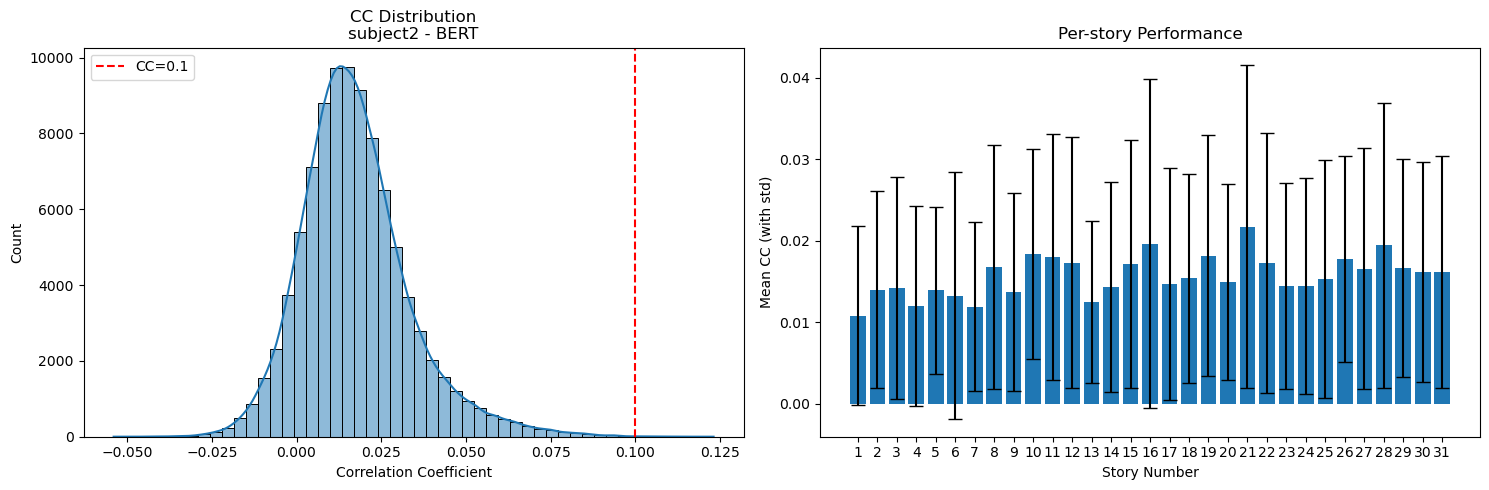
\includegraphics[width=0.8\textwidth]{bert_pretrained_sub2.png}
  \caption{Evaluation of the Ridge Model with pretrained BERT embedding on Subject 2}
  \label{fig:evaluation_ridge_bert_pretrained_subject2}
\end{figure}

\begin{figure}[H]
  \centering
  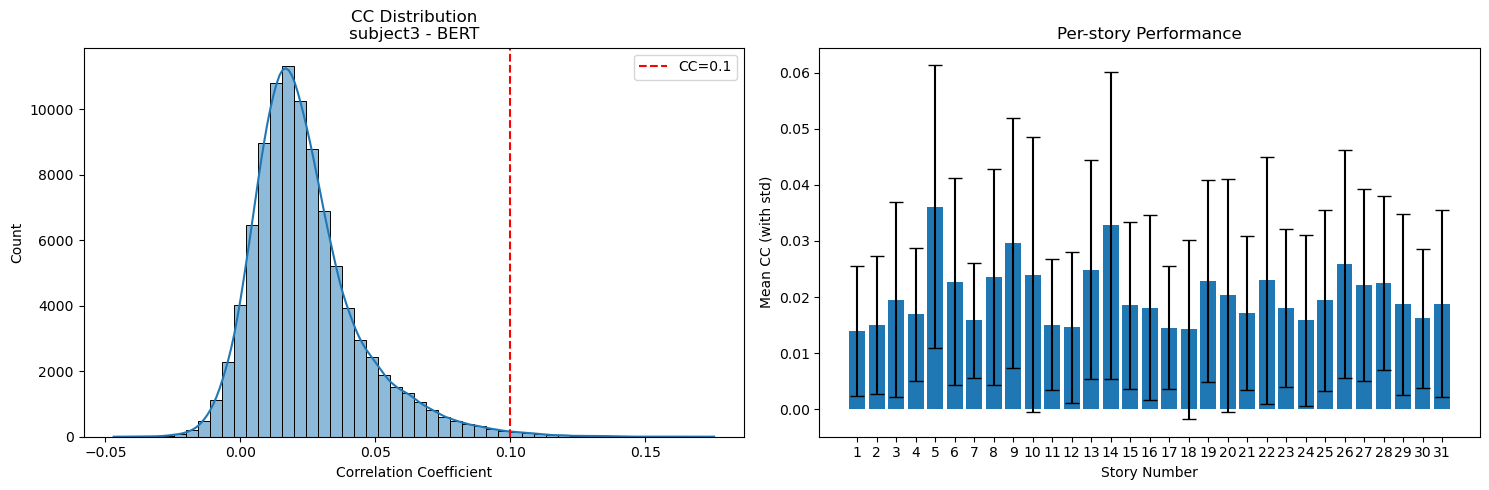
\includegraphics[width=0.8\textwidth]{bert_pretrained_sub3.png}
  \caption{Evaluation of the Ridge Model with pretrained BERT embedding on Subject 3}
  \label{fig:evaluation_ridge_bert_pretrained_subject2}
\end{figure}

\begin{figure}[H]
  \centering
  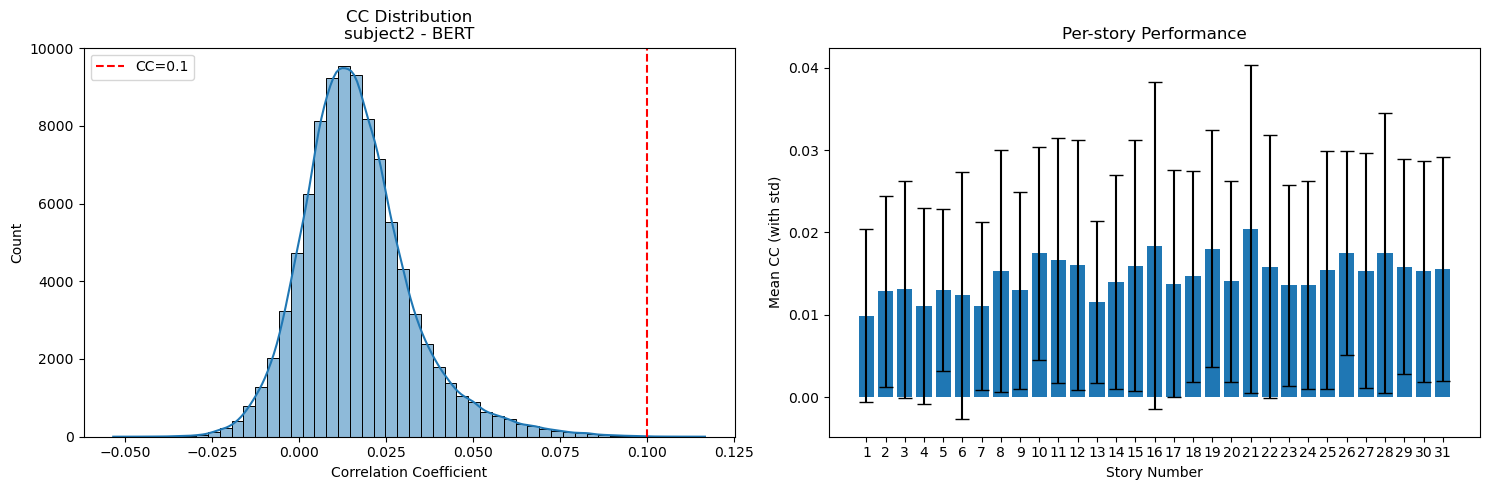
\includegraphics[width=0.8\textwidth]{bert_finetuned_sub2.png}
  \caption{Evaluation of the Ridge Model with finetuned BERT embedding on Subject 2}
  \label{fig:evaluation_ridge_bert_pretrained_subject2}
\end{figure}

\begin{figure}[H]
  \centering
  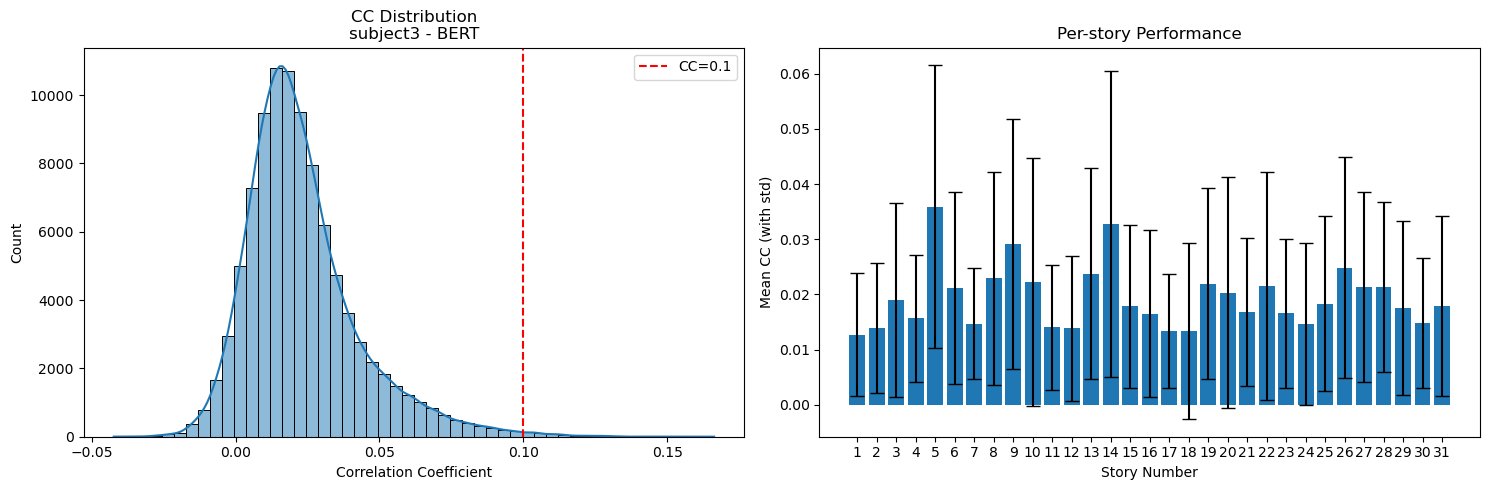
\includegraphics[width=0.8\textwidth]{bert_finetuned_sub3.png}
  \caption{Evaluation of the Ridge Model with finetuned BERT embedding on Subject 3}
  \label{fig:evaluation_ridge_bert_pretrained_subject2}
\end{figure}

\begin{figure}[H]
  \centering
  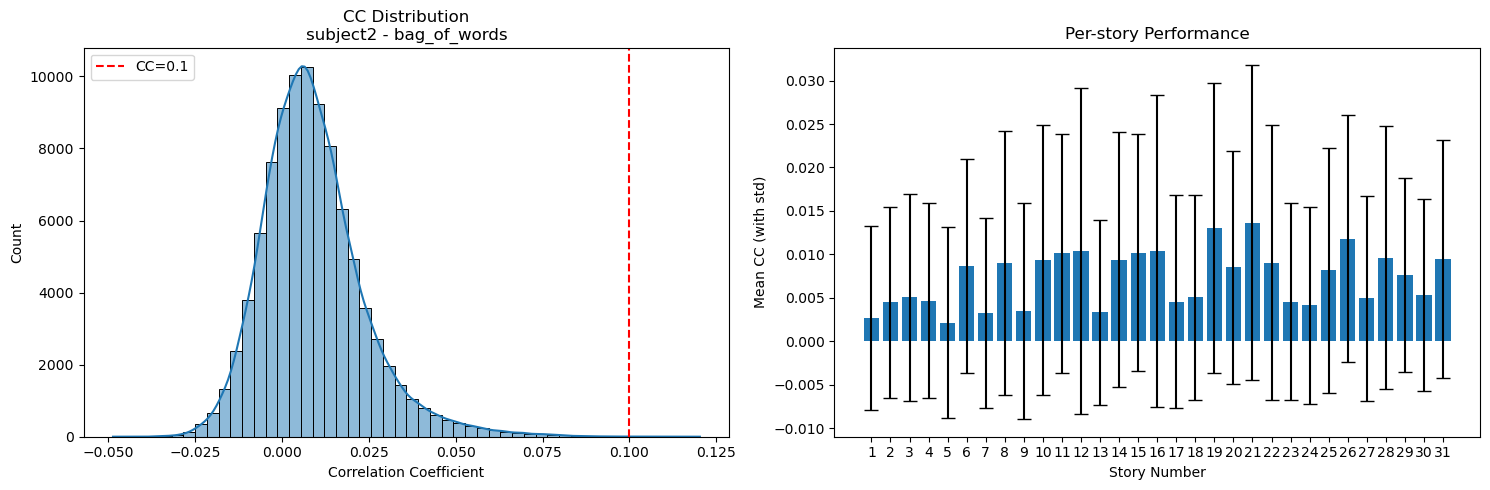
\includegraphics[width=0.8\textwidth]{bag_of_words_sub2.png}
  \caption{Evaluation of the Ridge Model with Bag-of-Words (in lab3.1) on Subject 2}
  \label{fig:evaluation_ridge_bert_pretrained_subject2}
\end{figure}

\begin{figure}[H]
  \centering
  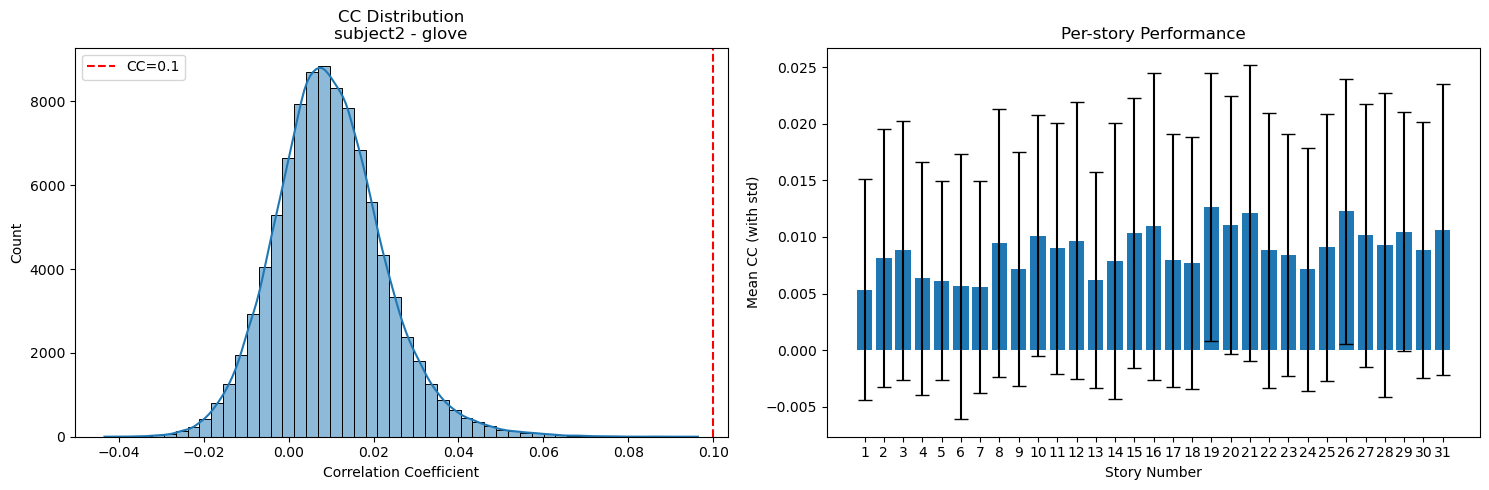
\includegraphics[width=0.8\textwidth]{glove_sub2.png}
  \caption{Evaluation of the Ridge Model with GloVe (in lab3.1) embedding on Subject 2}
  \label{fig:evaluation_ridge_bert_pretrained_subject2}
\end{figure}

\begin{figure}[H]
  \centering
  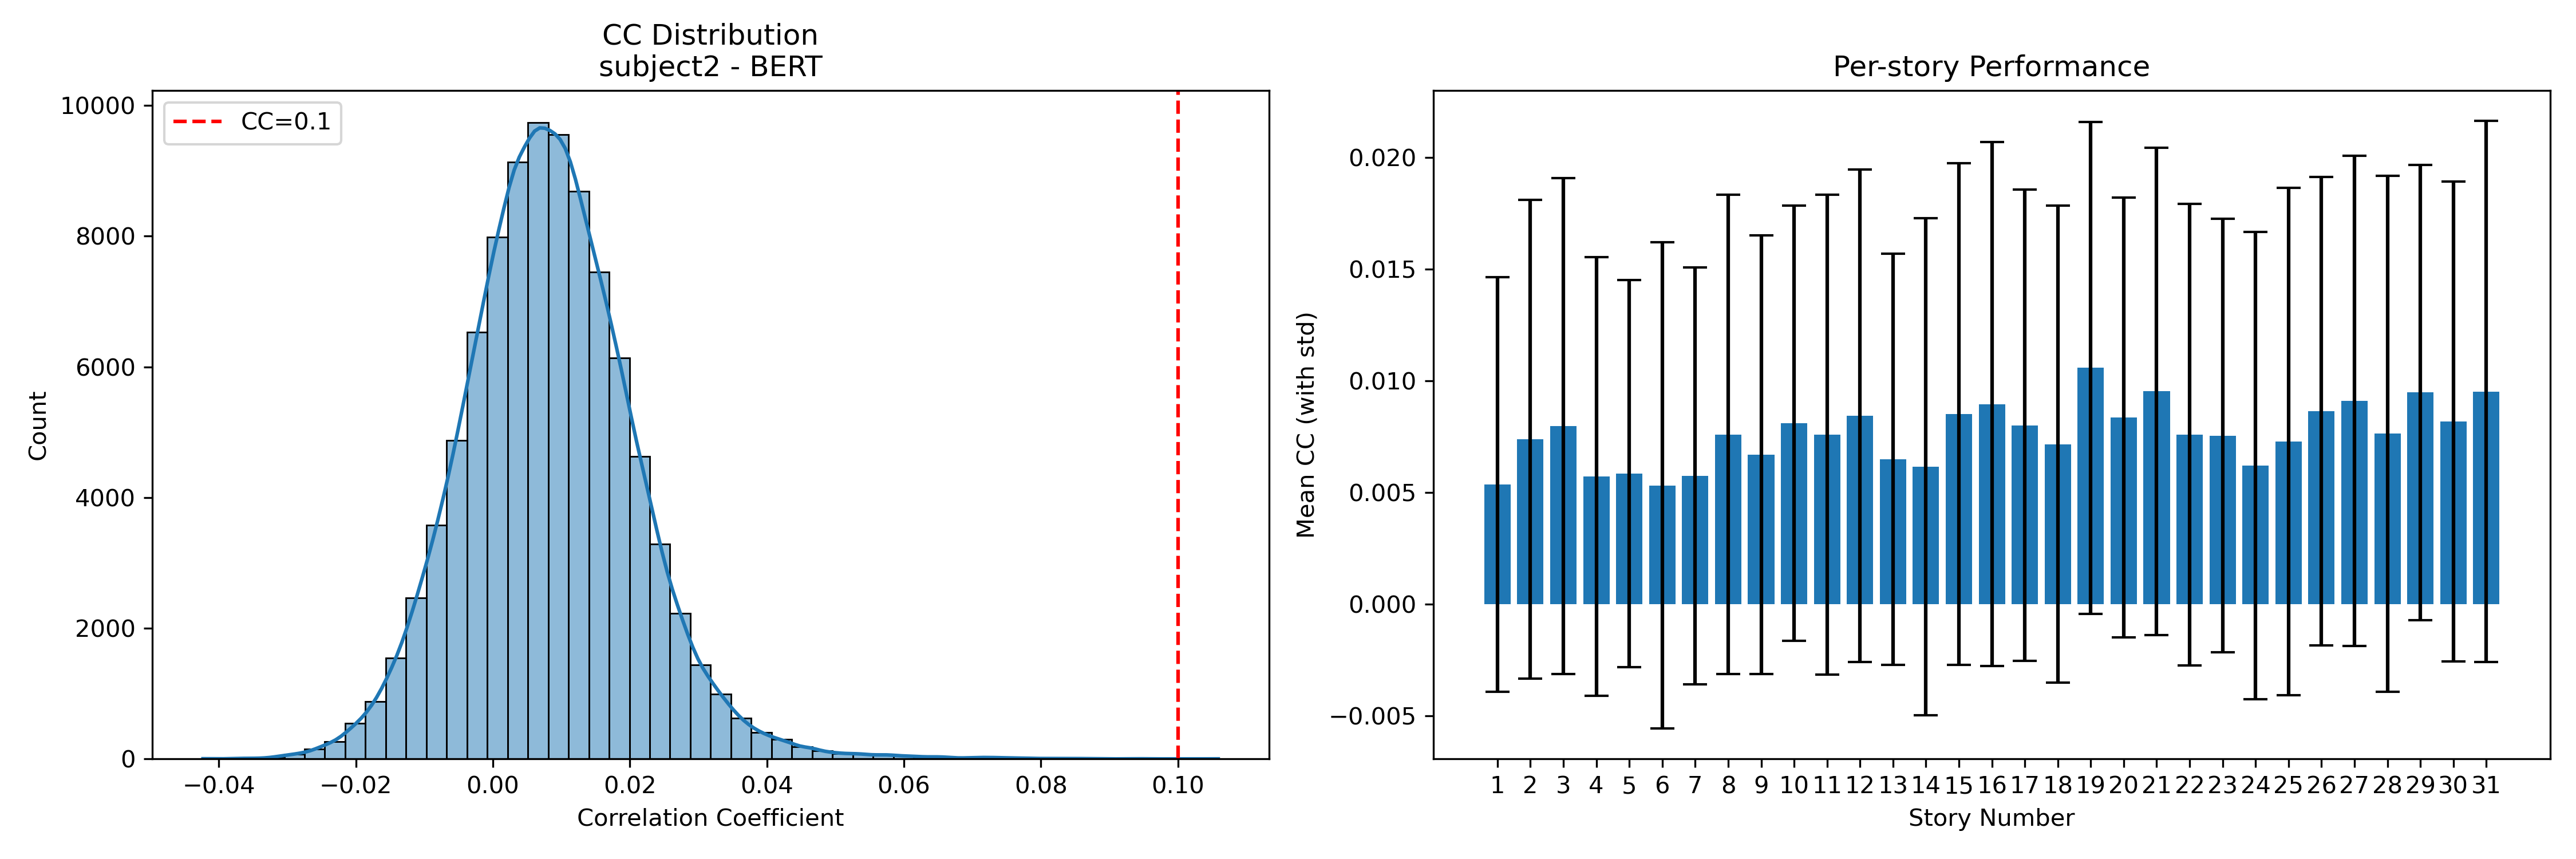
\includegraphics[width=0.8\textwidth]{bert_sub2.png}
  \caption{Evaluation of the Ridge Model with BERT (in lab3.2) embedding on Subject 2}
  \label{fig:evaluation_ridge_bert_pretrained_subject2}
\end{figure}

\section{Interpretation}

\subsection{General Methodology}
Based on the described BERT model, the ridge prediction and the results shown, we want to understand the model in more detail and interpret it from different perspectives. We will select two stories from the test data set and determine the voxel that was best predicted using the ridge model and use SHAP and LIME to look at the words that play a particularly important role. We restrict these explanations to voxels with strong predictive performance, reflecting the “P” (Predictivity) principle of the PCS framework. By focusing on voxels that are well predicted, we ensure that SHAP and LIME capture real stimulus–response relationships and not noise or artifacts of unreliable predictions.

The BERT model itself is a special feature. As a maximum of 500 words can be processed there, the prediction is determined in several batches, which are then merged again for the final result of SHAP and LIME.

\subsection{SHAP Overview}
SHAP (SHapley Additive exPlanations) is a game-theoretic framework for interpreting machine-learning predictions. The result is an additive explanation in which the model’s output for a single instance is decomposed into a baseline value (what the model would predict without information) plus a set of feature-specific contributions that sum exactly to the final prediction. In this lab, SHAP was used to interpret the predictions of voxel-specific ridge regression models trained on encoded text features. By treating each word in a passage as a potential contributor to the predicted neural activation for a given voxel, SHAP assigns importance scores that reflect how much each word increases or decreases the predicted response. To handle long texts exceeding the model input limit, we processed the input in overlapping chunks and aggregated SHAP values across them. This allowed us to identify which words most strongly influenced neural activity at specific voxels, providing insight into the semantic features driving brain responses in natural language comprehension.

\subsection{LIME Overview}
Local Interpretable Model-agnostic Explanations (LIME) is a post-hoc explanation method that provides explanations for the local predictions of any black-box model by generating small perturbations around one instance, querying the model, and constructing a sparse linear surrogate locally to approximate the decision boundary of the model. In contrast to SHAP, which utilizes Shapley values from cooperative game theory to give additive and consistent feature attributions for every instance, LIME focuses only on local fidelity and makes fewer estimates, producing typically faster but less consistent results. When used for text data, LIME indicates the words or phrases most accountable for pushing the model towards either class, allowing practitioners to find trigger tokens / words and show model behavior. This is why we also use it here, as it can be used to emphasize the influence of individual words on the final result.

\subsection{Test-Story 1: Tetris}
We have selected the Tetris story with the measured values from Subject 3 as the first test story. The voxels with the top 2 highest performance is voxel 127 and voxel 128. We will focus our results in this subsection on these two voxels. Other well-performing voxels have shown similar results.

\subsubsection{SHAP Test Story 1, Voxel 127}

In Figure 8, we can see SHAP results for voxel 127 of the test story, Tetris. 

\begin{figure}[H]
    \centering
    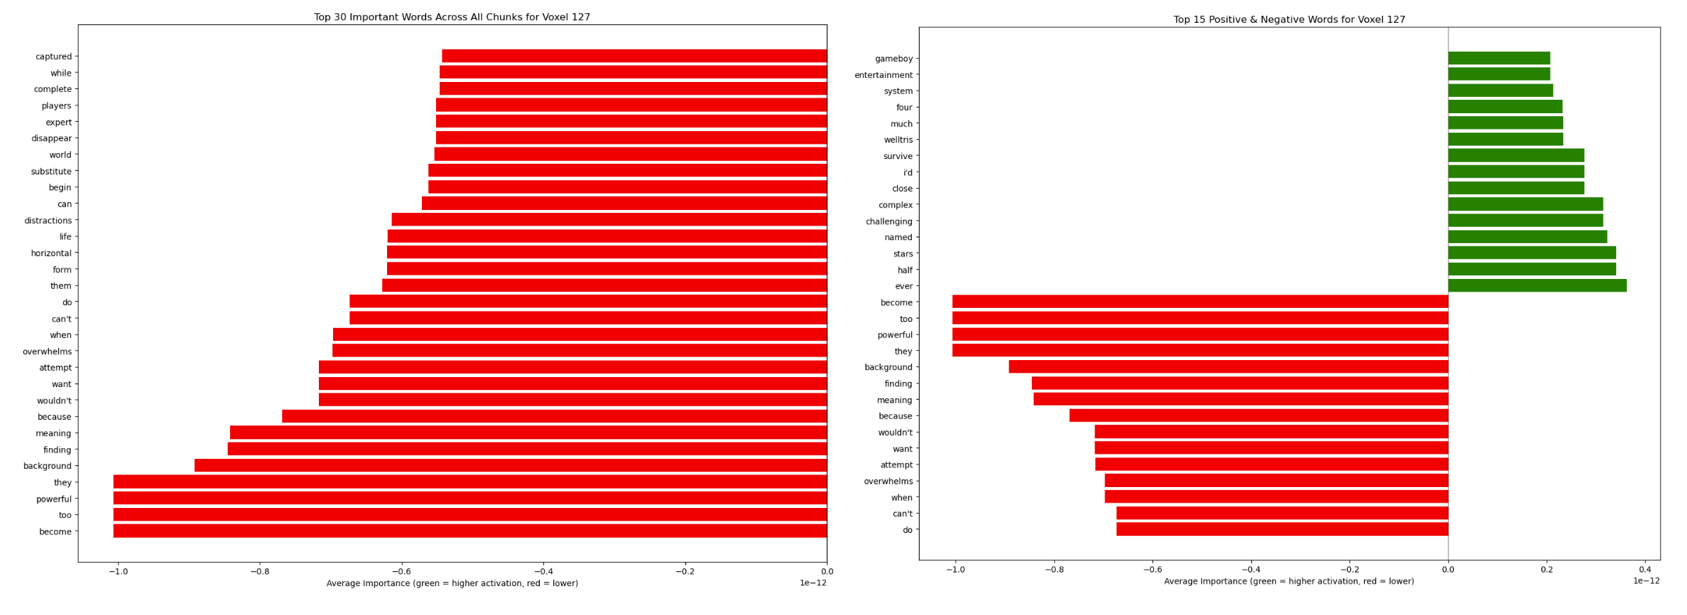
\includegraphics[width=1.0\linewidth]{shap_story1vox127.png}
    \caption{SHAP for Test Story 1, Voxel 127}
    \label{fig:enter-label}
\end{figure}

The green bars represent words that increase the predicted voxel activation and vice versa for red bars.  

From the left plot, can see that the top 30 most important words all have a suppressing effect of brain activity on the voxel 127 region. Specifically, 'become', 'too', 'powerful', and 'they' have the highest magnitude of all words in the test story. From the right plot, words with green bars such as 'gameboy', 'entertainment', and 'system' are thematically tied to video games and may trigger activity in regions related to visual processing, semantic memory, etc. In the red bars, we have words such as do, can't, attempt and overwhelms that are all associated with effort, failure, or difficulty which may be linked to cognitive control areas of the brain that suppress activity in voxel 127. 

Overall, voxel 127 seems to respond more to concrete ideas such as video games and less to negative concepts such as failure or effort. This may indicate that it plays a role in visual or semantic processing rather than in higher-level thinking or emotion. 

\subsubsection{LIME Test Story 1, Voxel 127}
In Figure 9, we can see the results of LIME for voxel 127 of the test story, Tetris.

\begin{figure}[H]
  \centering
  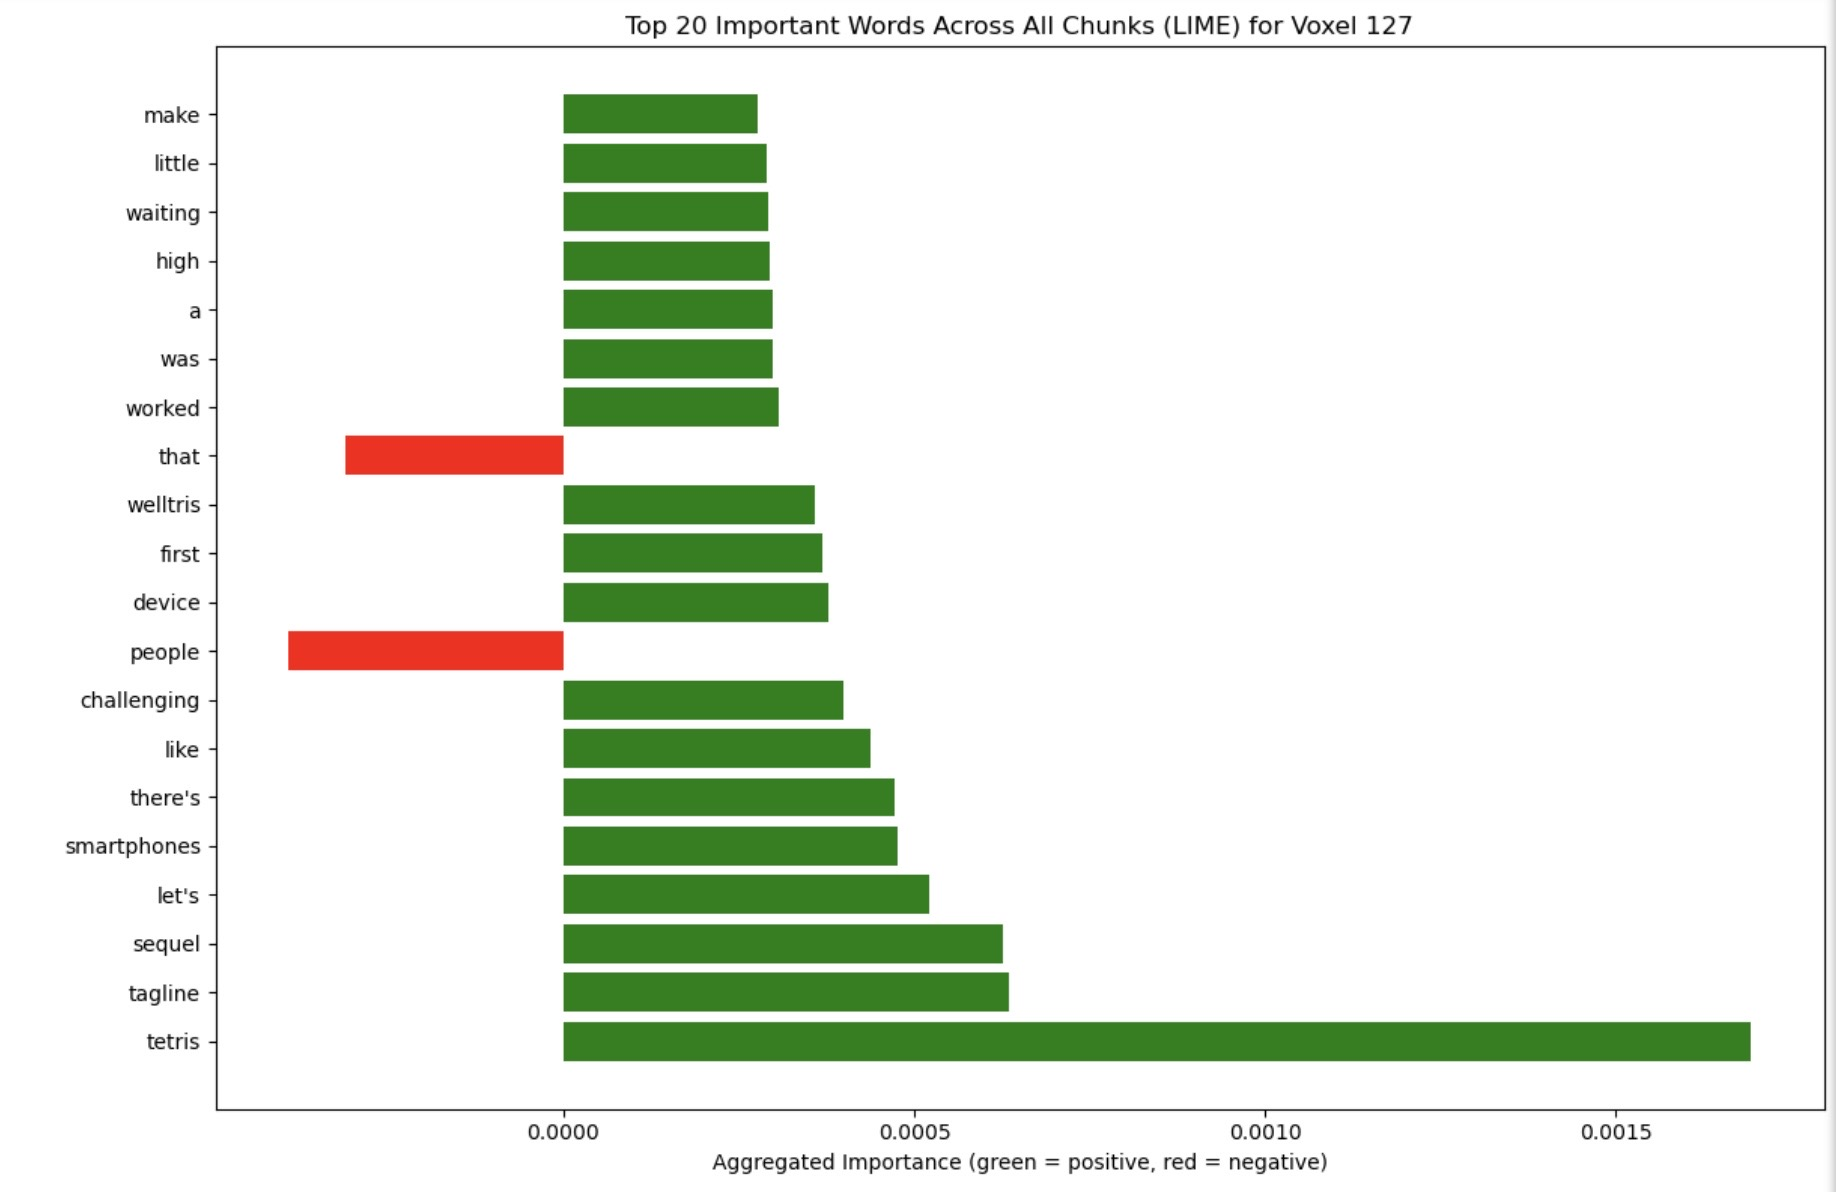
\includegraphics[width=0.8\textwidth]{LIME_Result_Test_Story_1_127.jpeg}
  \caption{LIME for Test Story 1 Voxel 127}
  \label{fig:LIME1}
\end{figure}

We can see that words such as 'tetris' (the main topic in the story) have a big impact and other words such as 'tagline', 'sequele', 'let's' or 'smartphones' also have a positive influence on the prediction. Other words such as 'people' and 'that 'tend' to have a negative influence on the prediction. This corresponds to a person's intuition, as many of the words are strong words at the heart of the story and a particularly strong reaction from the person is to be expected.

\subsubsection{SHAP Test Story 1, Voxel 128}
In Figure 11, we display the top words that influenced the predictive activation of voxel 128 based on SHAP values. The left plot shows the top 30 words and the right plots shows the top 15 words with positive and negative average SHAP values. 
We can see that words like 'programmer', 'worker', 'let's', 'start', and 'player' are associated with increased activation. These words are related to agency, planning, roles, or gaming. This suggests that voxel 128 is more active when the story involves goal-oriented or structured activity. From the right plot we see that words such as 'mess', 'courts', 'involved' and 'rich' lead to lower activation. These words are associated with complexity, conflict, or corporate themes. 

\begin{figure}[H]
    \centering
    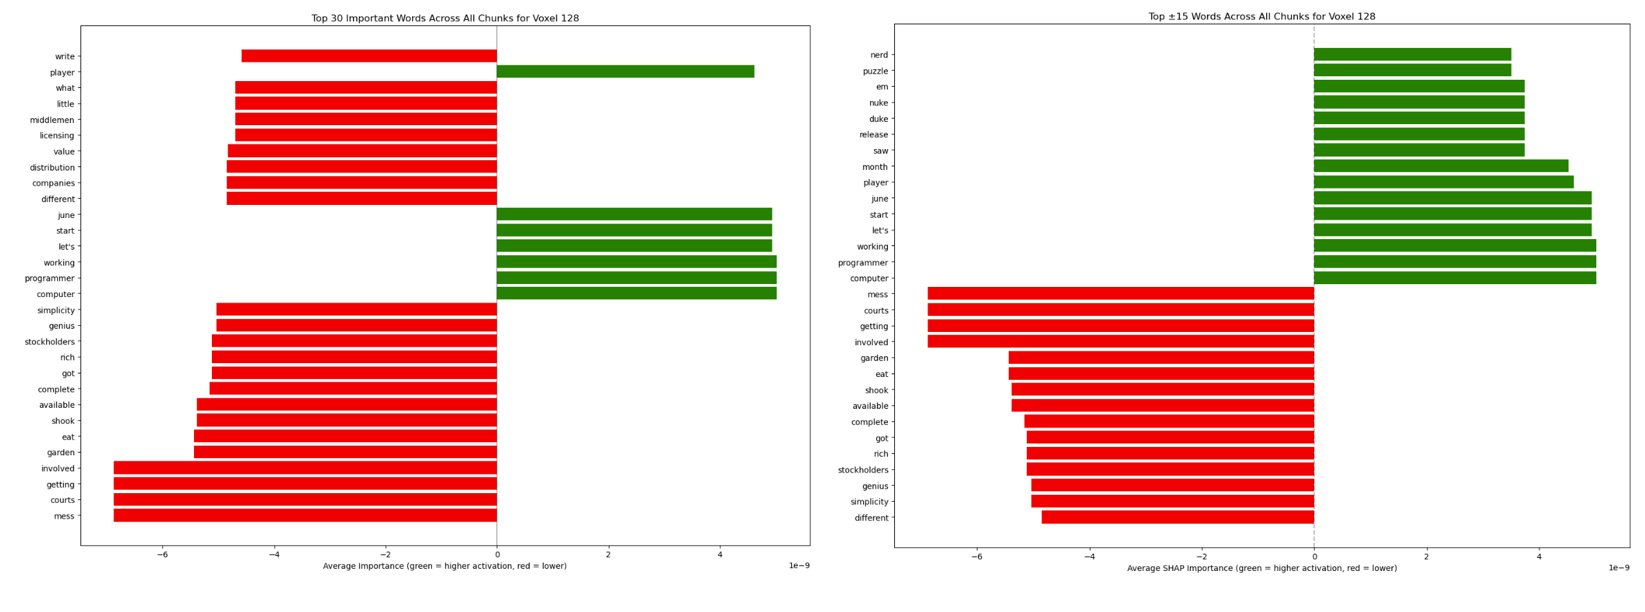
\includegraphics[width=1.0\linewidth]{shap_story1vox128.png}
    \caption{SHAP for Test Story 1, Voxel 128}
    \label{fig:enter-label}
\end{figure}

Overall, voxel 128 appears to be activated by goal-oriented or interactive language and suppressed by language related to social or organizational complexity. These patterns suggest that voxel 128 is a brain-region responsive to action-oriented thinking and less responsive to abstract or institutional concepts. 

\subsubsection{LIME Test Story 1, Voxel 128}
In Figure 11, we can see the results of LIME for the voxel 128:

\begin{figure}[H]
  \centering
  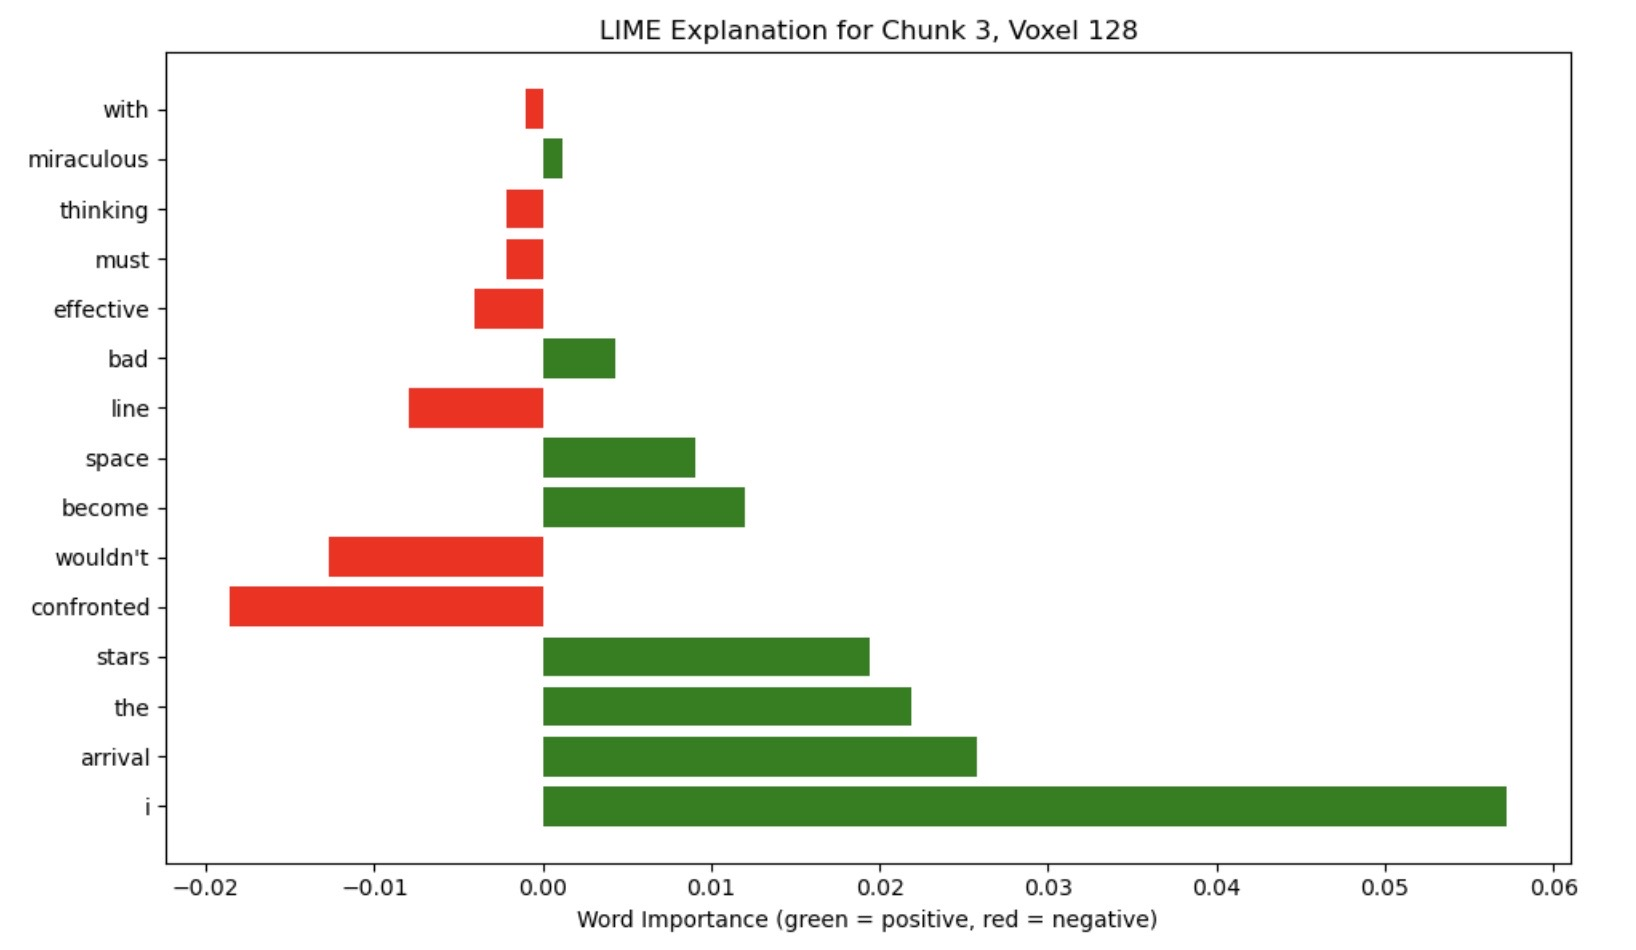
\includegraphics[width=0.8\textwidth]{LIME_Result_Test_Story_1_128.jpeg}
  \caption{LIME for Test Story 1 Voxel 128}
  \label{fig:LIME1}
\end{figure}

We can see that words such as 'i', 'arrival', 'the', and 'stars' have a positive influence on the prediction. Other words such as 'confronted' and 'wouldn't' tend to have a negative influence on the prediction. This corresponds in part to the expectation, although a connecting word such as ‘that’ cannot necessarily be considered particularly important from a human point of view.

\subsection{Test-Story 2}
We have selected the 'My Father's Hands' story with the measured values from Subject 3 as the first test story. We will focus on the voxel with the highest performance, voxel 143. Other well-performing voxels have shown similar results.

\subsubsection{SHAP}

From Figure 12, we can see that all of the top 30 words, ranked by the magnitude of their SHAP values, have negative SHAP values. In fact, every word in the story shows a negative SHAP value.   

Words such as 'whenever', 'anywhere', 'car', 'held', and 'touched' have the largest negative impact on voxel 143. These words mostly relate to movement, physical interaction, or emotional moments.  
This might suggest that voxel 143 is less responsive when processing emotionally charged or sensory language, especially involving people and physical space.   

In general, voxel 143 shows strong negative responses to words related to emotion and action. This suggests that the voxel is located in a brain-region that suppresses activity during emotional and physical contexts. 
The consistently negative SHAP values may imply that the voxel may be less involved in processing the narrative elements of 'My Father's Hands' which is a story centered on emotion and human connection. Alternatively, it may suggest the presence of subject-specific bias or systematic suppression in the voxel's response throughout the narrative. Intuitively, it is unlikely for all words in a story to have a suppressing effect on brain-region region activity due to the nature of a story (exposition, rising tension, climax, conclusion, etc).   

\begin{figure}[H]
    \centering
    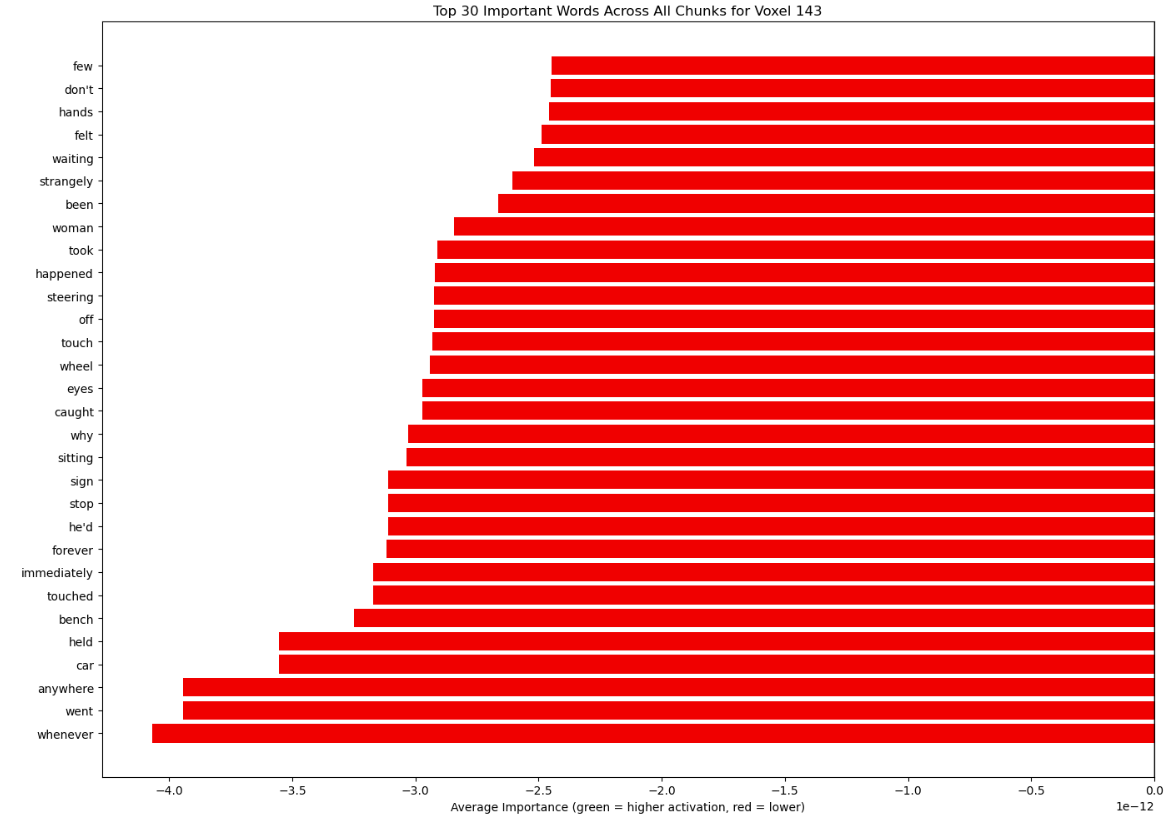
\includegraphics[width=0.5\linewidth]{shap_story2.png}
    \caption{SHAP for Test Story 2}
    \label{fig:enter-label}
\end{figure}


\subsubsection{LIME}
In Figure 13, we can see the results of LIME for the voxel 143:

\begin{figure}[H]
  \centering
  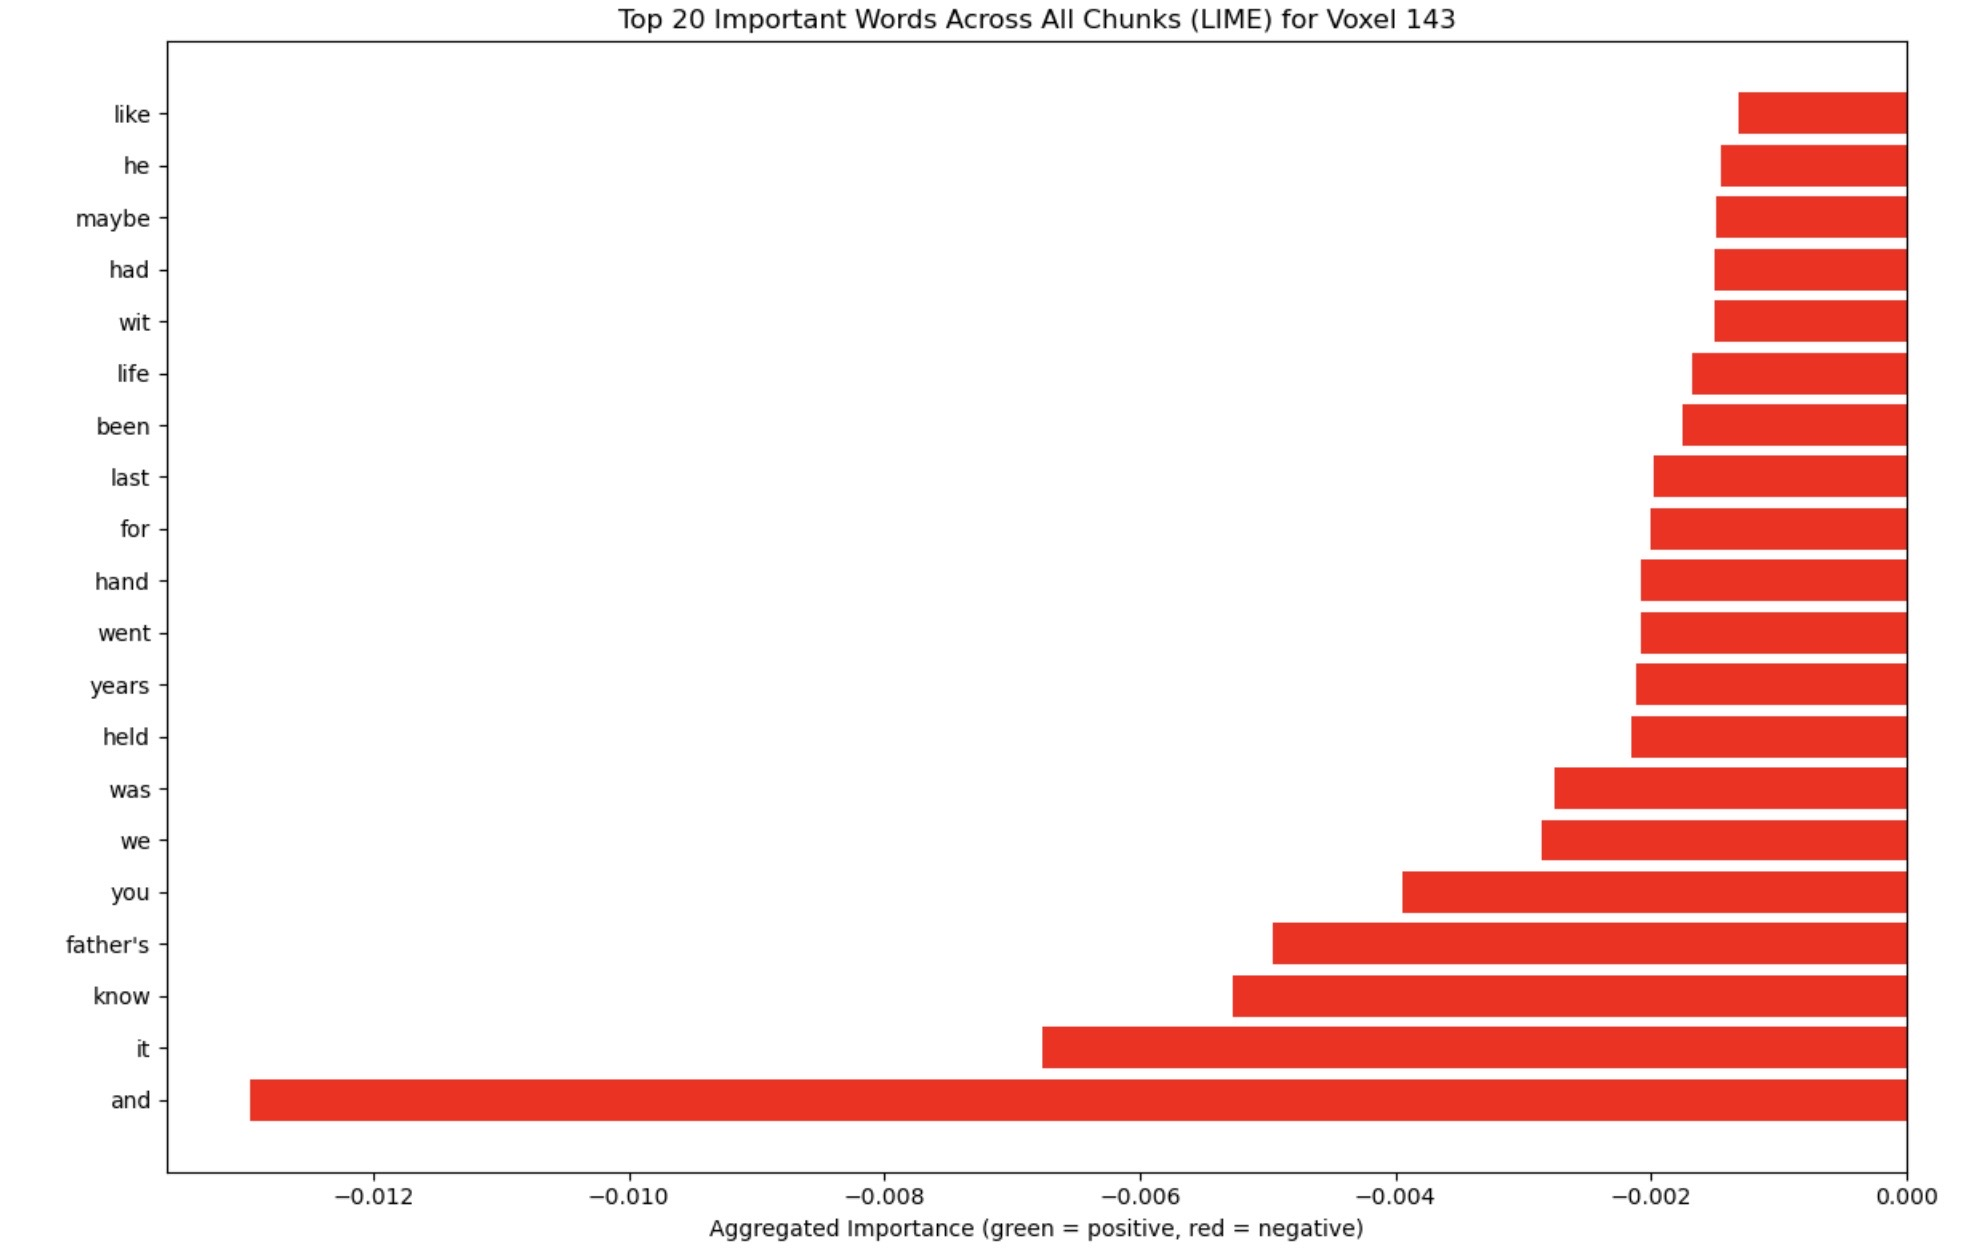
\includegraphics[width=0.8\textwidth]{LIME_Result_Test_Story_2_143.jpeg}
  \caption{LIME for Test Story 2 Voxel 143}
  \label{fig:LIME1}
\end{figure}

We can see that the text mainly contains words with a strong negative impact. The words 'and', 'it', 'know' and 'father's' have there the strongest negative incluence. It is difficult to clearly classify why the following words have a negative effect, as it is difficult to imagine a corresponding connection between the words.

\subsection{Comparisons between SHAP and LIME}
Overall, it can be seen from the voxels under consideration that the SHAP method identifies other words as relevant than the LIME method does. At the same time, it is not easy to interpret why individual words have a corresponding effect and other words do not. This means that we cannot confirm a person's intuition that there are “clear” important words that have a corresponding effect. At the same time, however, this must also be taken into account, as the performance is still not particularly good even with the best voxels and this can of course also lead to the results obtained from SHAP and LIME being distorted.

\section{Conclusion}

In this lab, we used pre-trained BERT models and fine-tuned it using LoRA to predict brain activity, and applied interpretation methods to understand brain-language relationships in fMRI data. Our results show that pre-trained BERT models significantly outperformed previous embedding methods (Bag-of-Words, Word2Vec, GloVe, and our Lab 3.2 BERT), achieving a higher correlation coefficients with brain activity. Fine-tuning with LoRA improved results slightly more, especially in terms of the mean CC of Subject 3.

We then used this finetuned model for embedding in order to train a ridge model for predicting the voxels, as we did in the previous labs and  tried to better understand the performance with the help of SHAP and LIME. The interpretation analysis with SHAP and LIME identified potentially important words for different voxels, though the patterns were not always easy to interpret and the two methods sometimes disagreed on which words were most important.

Overall, predicting brain activity from language is still very difficult. However, our work shows that pre-trained language models like BERT perform much better than previous methods. While we found some interesting patterns in how different brain regions respond to certain words, much work remains to be done.

\section{Bibliography}

Jain, Shailee, and Alexander Huth. “Incorporating Context into Language Encoding Models for FMRI.” 

\section{Collaborators} 

I certify that I have only collaborated with my group members. 


\section{Academic honesty}
To: Bin Yu 

I declare that the work presented in Lab 3.3 is entirely my own and my group members. We ourself designed and performed all the data analysis, methods and procedures presented in this report. We ourself wrote all the texts, wrote codes embeddings, modeling, and produced all the figures in this report. We used codes provided by GSI. We have included and documented all the procedures in the workflow and the results are fully reproducible. Wherever we included the work from others, we cited the sources and in 'References section', especially for equations. We used LLM specifically for improved grammar for report writing style.

By submitting this lab report and all github material, I certify that we have complied with the academic integrity standards as set in lab 3.3 instructions. 

\section{References}

\begin{itemize}

    \item \href{https://arxiv.org/abs/2106.09685}{LoRA}
    \item \href{https://docs.unsloth.ai/get-started/fine-tuning-guide/lora-hyperparameters-guide}{Hyperparameter Optimization for LoRA}

    
    
\end{itemize}


\end{document}
